%!TEX root = ../main.tex

\section{Optimizing the Basic Approach}
\label{sec:opt}

A large drawback of our basic MILP transformation (Section~\ref{sec:sol}) is
that it exhaustively encodes the combination of all tuples in the database and all queries
in the query log.  In this approach, the number of constraints (as well as undetermined variables) 
grows quadratically with respect to the database and the query log.
\ewu{Actually encoding all queries or only oldest query as undetermined variables.  The latter motivates the incremental optimiation in Section~\ref{sec:incremental}}
\ewu{Alternative: Just talk about red bars.  Blue bars discussed in incremental section}
Figure~\ref{fig:querysize_vs_time} shows a simple scalability experiment, where we generated increasingly 
larger query logs for a database of $1000$ tuples, encoded the problem using \naive (red bars), 
and solved the problem using a MILP-solver (CPLEX in our experiments).
We find that the solver time increases exponentially as the number of encoded queries increases --
at a log size of $80$, the solver failed to produce an answer within $1000$ seconds --
due to the exponential increase in the number of possible states for the increasing number of undetermined variables.
In contrast, the blue bar illustrates the near-constant performance of a similarly encoded but optimized MILP problem. 
% {\it only parameterizes the constants of the oldest query in the log}.
Although the empirical solver performance varies widely depending on the specific problem, 
this experiment illustrates the limitations of the na\"ive approach.

\begin{figure}[h]
    \centering
    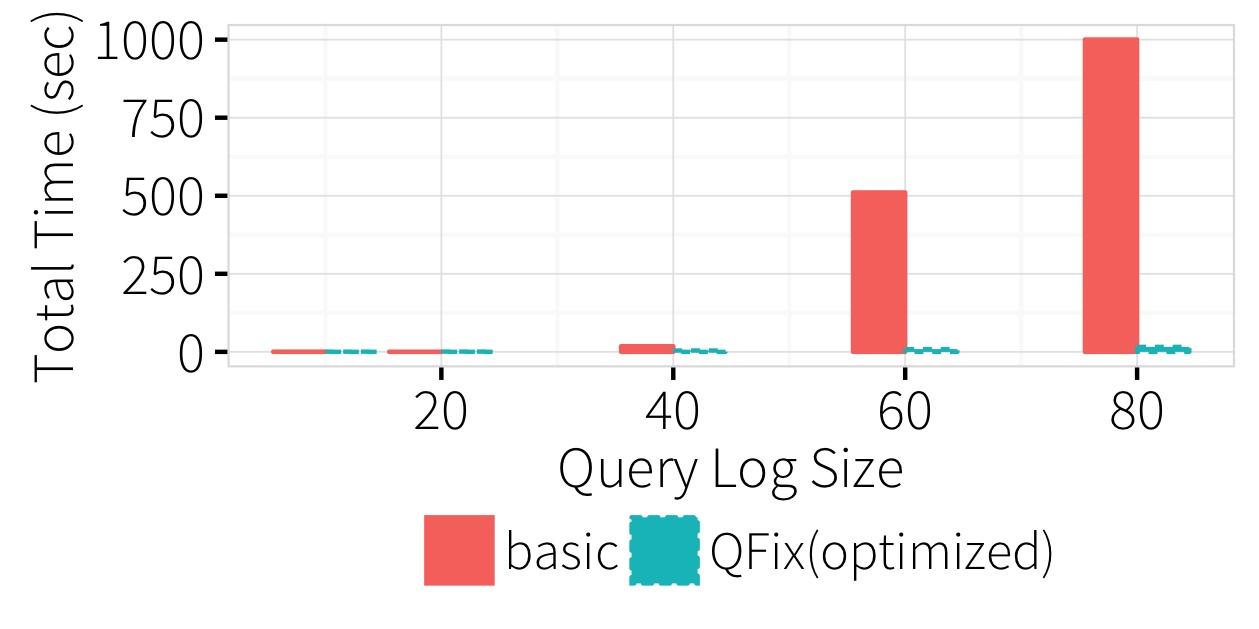
\includegraphics[width=0.35\textwidth]{figures/qsize_time_badscale}
    \vspace*{-0.1in}
    \caption{Log size vs. execution time on synthetic setup. }
    \label{fig:querysize_vs_time}
\end{figure}
\vspace*{-0.1in}

To resolve this limitation, we explored three classes of \emph{slicing} optimizations that seek to
reduce the number of tuples, queries, and attributes that are encoded in the MILP problem.
In addition, we propose an incremental algorithm that exploits the single bar performance observed
in the above scalability experiment, which both improves the scalability and the repair latency
when the corrupted query is recent.  




% In the previous section, we introduce the basic approach to derive
% the log repair by incorporating information from every query
% and every tuple into a single MILP problem. However, oftentimes, 
% this basic approach end up with 
% a huge problem as the query log size and table size increase. 
% In Figure~\ref{fig:querysize_vs_time}, 
% we observe that the total solver (IBM CPLEX) solving time 
% grows exponentially and 
% unpredictably as the query 
% log size or the table size increases. As a result, the basic approach does not scale over 
% large problems (large query log size and large table size).


\if{0}
linearize whole query log, so cost of adding an additional tuple is very high.
second iteration generally takes ~1 - 10%
for large databases knn cost is pretty high: ~

if the solver returns, it is always a super set of the clean range

only tuples modified by the fixed queries
- tuples already in the complaints (correct)
- not in complaints, but any of the originial queries modified it
- not in complaints, but no original queries modified it
\fi



\subsection{Reducing Tuples (Tuple Slicing)}
\label{sec:opt:tbsize}
\begin{figure}[t]
    \centering
    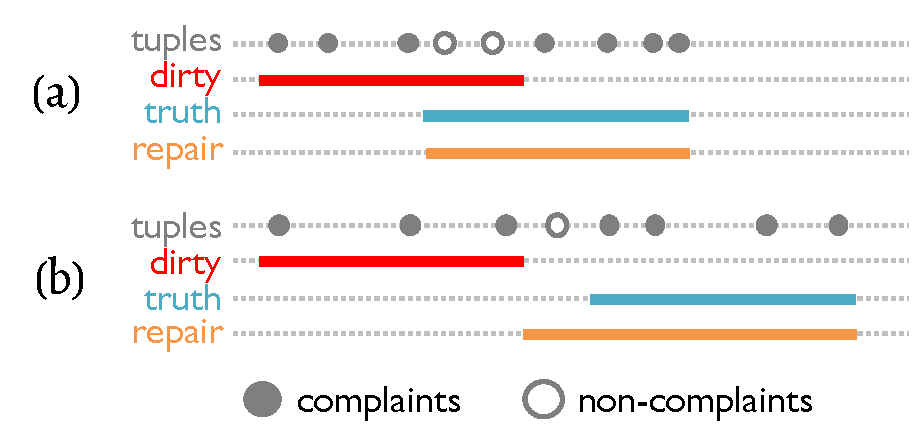
\includegraphics[width=0.35\textwidth]{figures/2nditerationgroups}
    \vspace*{-.2in}
    \caption{
      Graphical depiction of correct (a) and over-generalized (b) repairs.
      Solid and empty circles represent complaint and non-complaint tuples.
      Each thick line represents the interval of query $q$'s range predicate.
      Dirty: incorrect interval in corrupted query;
      truth: correct interval in true query;
      repair: interval returned by the solver.}
    \label{fig:groups}
    \vspace*{-.2in}
\end{figure}

% \ewu{Assume reader is clear that we are only repairing WHERE clause range predicates}
Our first optimization, \emph{tuple slicing}, applies a two step process to reduce the 
problem size without sacrificing accuracy: it
first aggressively reduces
the problem size by only encoding tuples in the complaint set and then refines the log repair 
through a second but much smaller MILP problem. 
\noindent\textbf{Step 1 (Initial Repair Step):} 
The first step of  \emph{tuple slicing} 
aggressively reduces the problem size by only encoding those 
tuples in the complaint set $\mathcal{C}$ (Algorithm~\ref{alg:basic} line $2$
is replaced with \texttt{for each t in $\mathcal{C}$}). 
Each tuple necessitates
the linearization of the entire query log, thus, only encoding the complaint tuples minimizes the 
size of the problem with respect to the relevant tuples. 
\ewu{Too Verbose?}
This optimization is guaranteed to resolve $\mathcal{C}$, thus depending on the properties of the non-complaint records, it can generate correct repairs
an order of magnitude faster without hurting the accuracy. 
In Figure~\ref{fig:groups}(a),
the solver will guarantee a repair interval that excludes the two left-most complaints, includes the two right-most complaints,
and minimizes the difference between the dirty and repaired intervals (due to the objective function).
This effectively pushes the repair's lower-bound towards that of the dirty interval.
This is a case where such a solution is correct, because the dirty and truth intervals overlap.
(Recall that we do not have access to the truth interval, and our goal is to reproduce the truth interval given $\mathcal{C}$ (solid circles) and the corrupted query.) 

However, this approach can also cause the repair to be a {\it superset} of the truth interval, and affect tuples not part of the complaint set
Figure~\ref{fig:groups}(b) highlights such a case where the dirty and truth intervals are non-overlapping, and the non-complaint record between them has been incorrectly included in the repair interval---{\it because the MILP problem did not include the non-complaint.}
% where this aggressive approach generalized incorrectly.
% The dirty and clean intervals are non-overlapping, so the non-complaint tuple shown is not modified by $q$ (otherwise it would be a complaint!). This tuple is incorrectly included in the repaired interval, 
% \emph{because the MILP formulation does not constrain its value}.


% For example, in Figure~\ref{fig:groups}(a), the dirty and truth intervals overlap, thus the non-complaint tuples 
% within the overlapping region are correctly modified by the dirty interval. 
% In this case, the proposed repair correctly contains the non-complaint tuples and the algorithm is successful.\\
% \indent However, sometimes the problem may overfit 
% and not generalize to the entire database.
% Specifically, there are problem settings where the repaired range predicate in a query's \texttt{WHERE} clause is a superset of the true range 
% predicate, and introduces new errors by affecting tuples not originally part of  the complaint set. 
% Figure~\ref{fig:groups}(b) highlights such a case where this aggressive approach generalized incorrectly.
% The dirty and clean intervals are non-overlapping, so the non-complaint tuple shown is not modified by $q$ (otherwise it would be a complaint!). This tuple is incorrectly included in the repaired interval, \emph{because the MILP formulation does not constrain its value}.

\indent In both of these cases, the objective function will ensure that the repair
does not over-generalize the upper bound towards the right because that strictly increases the objective function.
%On the other hand, over-generalizing the lower bound towards the dirty interval
%is expected because it decreases the Manhattan distance between the repaired and corrupted lower bounds,
%which are parameters in the objective function. 
Therefore, our main concern is to refine the repair interval to exclude those non-complaint tuples in case (b).
Note that in the case of incomplete complaint sets, the user may opt to no execute the refinement step if she believes
that the non-complaint records are indeed in error.

%, to perform tuple slicing successfully, we need to reduce the repaired interval and exclude those non-complaint tuples in case (b).  
\smallskip

\noindent\textbf{Step 2 (Refinement Step):} 
Although there are many possible mechanisms to refine the initial repair (e.g., incrementally shrinking
the repaired interval until the non-complaint tuples are all excluded), 
the straightforward approaches are not effective when multiple corrupt 
queries have been repaired because they don't take the query interactions into account.

Instead, we solve this using a second, significantly smaller, MILP problem.   
Let $\mathcal{Q}^*_{rep}$ be the set of repaired queries from the  initial MILP formulation with tuple slicing;
$\mathcal{NC}$ be the set of non-complaint tuples now matching the repaired \texttt{WHERE} clauses, as in Figure~\ref{fig:groups}(b);
and $\mathcal{C}^+ = \mathcal{C} \cup \mathcal{NC}$.
We create a new MILP using $\mathcal{C}^+$ as the complaint set, and fix the values of all queries not in $\mathcal{Q}^*_{rep}$ to their assignment in the solution from the first step.
This ensures that only repaired query parameters can be perturbed, which vastly reduces the number of undetermined variables in the problem.
We further modify the objective function to only penalize the number of non-complaint tuples 
$t \in \mathcal{C}^+$  that are matched by the queries in $q \in \mathcal{Q}^*_{sub}$.
These selections are represented by the binary variable $x_{q, t}$, thus the updated objective function
is $\sum_{q \in \mathcal{Q}^*_{sub}} \sum_{t \in \mathcal{NC}} x_{q,t}$.

% % \alex{I don't think this is true; it doesn't interfere with incomplete complaints, but it is not a mechanism to solve them.}
% We use this same mechanism to address incomplete complaint sets.
In our experiments, we find that this second MILP iteration adds
minimal overhead ($0.1-0.5\%$) with respect to the initial MILP
problem, making \tslice an effective method to improve the performance of the basic approach, without compromising accuracy.

% \ewu{Need to clarify that the solver is a black box, who knows what goes on there.  Maybe where we introduce MILP-solvers}
% \xlw{The number of noncomplaints differs case by case. }


% Although the query log is linearized in the same fashion as the above tuple slicing optimization,
% we additionally include the non-complaint tuples that are selected by the repaired queries in the problem.
% We then set the value of all of the variables to the results of the 
% We then updae the objective function so
% 
% we dramatically reduce the number of undetermined variables and use a different objective function.
% We fix all of the undetermined variables e
% 
% The simple approach 
% Let $\mathcal{Q}^*_{sub}$ be the set of repaired queries.
% We first construct a set of constraints by linearizing the queries in the query log
% between the least and most recent queries in $\mathcal{Q}^*_{sub}$ with respect to $\mathcal{C}$.
% The key difference is that we repair all of the undetermined variables for $x$ in Equation~\ref{}
% based on the solutions to the first MILP problem.  
% In addition, we call $Linearize$ for each non-complaint tuple in the repaired interval.
% The objective function is to minimize the sum of the undetermined $x$ variables in the encoded
% problem.
% 

% fix is always the smallest possible, so it can only require a sceond iteration if the dirty and clean
% ranges don't overlap at all.  
% 
% The basic solution, which suggests to linearize every tuple in the database into the MILP problem,
% has two major disadvantages: 1. the system may end up with a large MILP problem that requires 
% the solver to run forever to solve; 2. we can only linearize the every tuple
% when the complaint set is complete, which is often hard to guarantee. Thus, in the first 
% optimization, we propose a two-iteration approach handles both of these two problems 
% by linearizing tuples in the complaint set in
% the 1st iteration and refining the log repair in the 2nd iteration. \\
% \subsubsection{1st iteration}
% We use tuples in the complaints $\mathcal{C}$ to construct the MILP problem and derive a 
% inaccurate log repair $\mathcal{Q}^*$\xlw {we need to find a term for this}. This inaccurate 
% log repair resolves tuples in the complaints $\mathcal{C}$, but, at the same time, 
% introduces noises by over correcting tuples that are not involved in the MILP problem. 
% As shown in Example~\ref{ex:2nditer}, by resolving tuples in complaints $\mathcal{C}$, 
% the system derives a log repair that introduces other errors. 
% \begin{example}\label{ex:2nditer}
% Including tuples in the complaints $\mathcal{C}$ to solve problem in Example~\ref{ex:taxes2} 
% and using Euclidean distance of variables in the query as the objective function, the system 
% derives a log repair $\mathcal{Q}^*$ with $q_1^*=$ \texttt{\small UPDATE Taxes SET rate = 30}
% \texttt{\small WHERE income >= \color{red}{9500.0001} \color{black}{and income <=} \color{red}{90000}}. 
% This log repair resolve tuples in the complaints. However, the fixed query $q_1$ has a much wider range 
% and it it incorrectly modifies tuples that are not in the complaint, e.g., tuple $t_4$.
% \end{example}
% \ewu{why would this happen if we encoded all the tuples?  Doesn't the objective penalize this case?}
% 
% 
% To avoid introducing such noises, we introduce the 
% 2nd iteration which targets on refining the log repair derived in 
% the 1st iteration. 
% \subsubsection{2nd iteration}
% The goal for 2nd iteration is to optimize the impact of the log repair (tuples
% modified by $\mathcal{Q}$). 
% Let $\mathcal{Q}^*_{sub} = \mathcal{Q}^*-\mathcal{Q}$ as 
% queries modified in the log repair, in the 2nd iteration, we 
% construct a separate MILP problem by linearizing 
%  queries between the first and the last query in
% $\mathcal{Q}^*_{sub}$, parameterizing variables in 
% the where clause for queries in $\mathcal{Q}^*_{sub}$,
% and maximizing the log repair impact score. 
% 
% 
% We define the impact score by dividing the 
% impacted tuples $T$ into three groups and defining the 
% impact score accordingly. \xlw {we need to fix these terms}. 
% 
% \smallskip
% 
% \noindent\textbf{Group 1}: tuples in the complaints $\mathcal{C}$. Impact of 
% $\mathcal{Q}^*$ on this group
% are guaranteed as correct. \textbf{Rule:} 
% strictly satisfy, including these tuples as 
% constraints in the 2nd iteration MILP problem. 
% 
% \smallskip
% 
% \noindent\textbf{Group 2:} tuples not in $\mathcal{C}$, but also modified 
% by the original query log $\mathcal{Q}$. Impact of $\mathcal{Q}^*$ 
% on the group 2 are likely to
% be correct. \textbf{Rule:} adding these tuples into the 
% rewarded tuple set $T_{reward}$. 
% \ewu{what does "modified by the original query log Q mean?}
% 
% \smallskip
% 
% \noindent\textbf{Group 3:} tuples not in $\mathcal{C}$ and not modified 
% by the original query log $\mathcal{Q}$. Impact of 
% $\mathcal{Q}^*$ on the last group should penalized, thus 
% we put them into $T_{penalize}$ (\textbf{Rule}).
% 
% \smallskip
% 
% The impact score, which is also the objective function for
% the MILP problem, is $T_{reward} - T_{penalize}$. \ewu{what exactly is this objective function?  the number of tuples modified?}We further 
% optimize the 2nd iteration to reduce the size of $T$ 
% by searching for K-nearest-neighbors
% of tuples in complaints $\mathcal{C}$. 
% There are multiple benefits for the two-iteration approach:
% \begin{itemize}
% \item It minimizes the size of MILP problem in the 1st iteration. 
% \item It refines the log repair while avoid over correcting tuples not in 
% the complaints $\mathcal{C}$. 
% \item It pptimizes the impacted tuples efficiently by controlling the queries 
% and number of impacted tuples
% involved in the 2nd MILP problem.
% \item In addition, it handles cases when we don't have complete complaints
% $\mathcal{C}$ (false negatives). 
% \end{itemize}




\if{0}
  \subsubsection{A Naive but Flawed approach}
  \ewu{Better explained as: CPLEX searches through an exponential space of all possible combinations of MILP variables.  In a chunked approach, the solution of each chunk is one out of a potentially arbitrary number of possible solutions, thus it is easy to pick an incorrect one}
  A natural idea to optimize the basic approach is 
  to \textbf{chunk the query log} into
  smaller, fixed size pieces and then solve each piece at a time: starting
  from the most recent piece, the system linearizes and parameterizes queries 
  in the current piece and derives a corresponding log repair; 
  it then examines the other pieces iteratively
  in the same way. Since complaints only provides
  true values for the most recent database state, in order to avoid 
  linearizing additional queries, 
  we need to know \textbf{rollback} the true values of tuples 
  until the last query in each query log piece. \\
  However, rollback the database is non-easy. An ideal, precise rollback
  algorithm would generate a set of valid ranges for each attribute of a tuple. 
  But the size of valid ranges also grows exponentially with the number queries
  we want to rollback, which, in turn, could not improve the system performance. 
  On the other hand, an approximate, imprecise 
  rollback algorithm would either make the rest of the problems
  infeasible to solve (only maintain fixed number of valid ranges) 
  or result in deriving 
  incorrect log repairs (maintain the lower 
  bound and upper bound among all valid ranges).
    

  In order to improve the system performance without losing accuracy, we propose
  the following two optimizations: query-slicing optimization 
  based on provenance over queries and
  attribute-slicing optimization based on provenance over 
  attributes. 
\fi





\subsection{Reducing Queries (Query-Slicing)}
\label{sec:opt:query}


In practice, many of the queries in the query log could not have affected the \emph{complaint attributes} (defined below). For example, if $q_{N-1}$ and $q_{N}$ 
only read and wrote attribute $A_1$, then they could not have contributed to an error in $A_2$.  
However, if $q_{N}$  wrote $A_2$, then either or both queries may have caused the error. 
In short, if we model a query as a set of attribute read and write operations, those 
not part of the causal read-write chain to the \emph{complaint attributes} can be ignored.
This is the foundation of our \emph{query-slicing} optimization.

% The exhaustive parameterization of all queries in the query log, as described
% in the basic approach, is typically unnecessary because many queries in the log
% could not have affected the tuple attribute values in the complaint set.
% To avoid such redundant computation, \textit{query-slicing} 
% removes \texttt{UPDATE} queries whose \texttt{SET} clauses did not modify 
% attributes that could possibly have affected the {\it complaint attributes} 
% specified in the complaint set.

\begin{definition} [Complaint Attributes $\mathcal{A}(\mathcal{C})$]
	The set of attributes identified as incorrect in the complaint set.
	\[\mathcal{A}(\mathcal{C}) = \{A_i | t.A_i \neq t^*.A_i, c(t,t^*) \in \mathcal{C}\}\]
\end{definition} 


\begin{definition}[Query dependency \& impact]
    Query $q_i$ has \textbf{direct-impact}, $\mathcal{I}(q_i)$, which is
    the set of attributes updated in its modifier function $\mu_{q_i}$
    (e.g., \texttt{SET} clause). Its \textbf{dependency},
    $\mathcal{P}(q_i)$, is the set of attributes involved in its
    condition function $\sigma_{q_i}$.
    
    We derive the \textbf{full-impact}, $\mathcal{F}(q_i)$, of a query $q_i$ by propagating its direct impact through subsequent queries in the log (Algorithm~\ref{alg:fullimpact}):
    \[
    \mathcal{F}(q_i)=\mathcal{I}(q_i)\bigcup_{\substack{j=i+1\\ \mathcal{F}(q_i)\cap \mathcal{P}(q_j) \neq \emptyset}}^n \mathcal{F}(q_j)
    \]
  % \begin{enumerate}
  %   \item The \textbf{dependency}, $\mathcal{P}(q)$, of a query $q$
  %   is the set of attributes involved in the condition function $\sigma_q$.
  %   %\[\mathcal{P}(q) = \Pi_{f_{q}.\sigma}(R)\]
  %   \item The \textbf{direct-impact} of query $q$, 
  %   $\mathcal{I}(q)$, is the set of attributes 
  %   updated in the modifier function $\mu_q$ 
  %   (e.g., \texttt{SET} clause).
  %   %\[\mathcal{I}(q) = \Pi_{f_{q}.\mu}(R)\]
  %   \item The \textbf{full-impact}
  %   of $q$, $\mathcal{F}(q)$, propagates $q$'s direct impact through
  %   the subsequent queries in the query log to collect {\it all} attributes
  %   that are affected by the changes caused by $q$'s update function.
  %   We describe its implications and computation below and in Algorithm~\ref{alg:fullimpact}.
  % \end{enumerate}
\end{definition}

% By comparing $\mathcal{F}(q)$ and $\mathcal{A}(C)$, we know whether
% or not corrupting query $q$'s parameters could possibly have caused the complaint
% set.  

% Algorithm~\ref{alg:fullimpact} describes how $\mathcal{F}(q_i)$ can be computed:
\begin{algorithm}[t]
\scriptsize
\caption{$FullImpact$ algorithm for finding $\mathcal{F}(q)$.}
\label{alg:fullimpact}
\begin{algorithmic}[2]
\REQUIRE {$\mathcal{Q}$, $q_i$}
% \ENSURE {$\mathcal{F}(\mathcal{Q})=\{\{\mathcal{F}(q_1)\}, ..., \{\mathcal{F}(q_n)\}\}$}
% \FOR {each $q_i$ in $q_n, ..., q_1$}
\STATE $\mathcal{F}(q_i) \leftarrow \mathcal{I}(q_i)$
\FOR {each $q_j$ in $q_{i+1}, ..., q_{n} \in \mathcal{Q}$}
\IF {$\mathcal{F}(q_i)\cap \mathcal{P}(q_j) \neq \emptyset$}
\STATE $\mathcal{F}(q_i) \leftarrow \mathcal{F}(q_i) \cup \mathcal{F}(q_j)$
\ENDIF
\ENDFOR
%\STATE $\mathcal{F}(\mathcal{Q}) \leftarrow \mathcal{F}(\mathcal{Q}) \cup {\red{\{\mathcal{F}(q_i)\}}}$
% \ENDFOR
\STATE Return $\mathcal{F}(q_i)$
\end{algorithmic}
\end{algorithm}
\vspace*{-.1in}

By computing the full-impact of $q$, we can determine the extent that it affects $\mathcal{C}$
based on its overlap with the complaint attributes.
Specifically, 
when $|\mathcal{F}(q) \cap \mathcal{A}(C)|=|\mathcal{A}(C)|$, $q$ may affect all complaint attributes and is a candidate for repair; 
when $0 < |\mathcal{F}(q) \cap \mathcal{A}(C)| < |\mathcal{A}(C)|$, 
$q$ contributed to a subset of the complaint attributes and is a candidate for repair;
when $|\mathcal{F}(q) \cap \mathcal{A}(C)|=0$, $q$ is irrelevant 
and can be ignored during the repair process.
We distinguish between the first and second conditions in the special case where we are repairing a \emph{single} 
corrupted query in the query log.  In this case, only queries in the first conditions are candidates for repair because 
the single query must have caused errors in all of the complaint attributes.  This enables \sys to scale significantly better
for this important problem setting. 
Finally, we use $Rel\mathcal{(Q)}$ to denote the set of relevant
queries that are candidates for repair. Our \emph{query slicing}
optimization, \qslice, linearizes only the queries in
$Rel\mathcal{(Q)}$, rather than the entire log, resulting in
smaller problems than \naive, without any loss of accuracy.

\subsection{Reducing Attributes (Attribute Slicing)}

In addition to removing irrelevant queries, we additionally avoid encoding irrelevant attributes.
Given $Rel\mathcal{(Q)}$, the relevant attributes can be defined as:
$Rel\mathcal{(A)} = \cup_{q_i \in Rel\mathcal{Q}} (\mathcal{F}(q_i)\cup \mathcal{P}(q_i))$
\aslice uses \emph{attribute slicing} to only encode constraints for attributes in $Rel\mathcal{(A)}$.
We find that this type of slicing can be effective for wide tables along with queries that focus on a small subset of attributes, such as TPC-C style transaction workloads. 
% \ewu{BAD TEXT!!!: However, our experiments on synthetic workloads show that this optimization is not useful in many settings, and most improvements are achieved by slicing on the tuple and query dimensions.}




\subsection{Single Query Incremental Repairs}\label{sec:incremental}

\begin{algorithm}[t]
\caption{\incremental algorithm. 
}
\scriptsize
\label{alg:incalg}
\begin{algorithmic}[2]
\REQUIRE {$Rel\mathcal{(Q)}, \mathcal{D}_j, \mathcal{D}_n, \mathcal{C}$}
\STATE Sort $Rel\mathcal{(Q)}$ from most to least recent
\FOR {each $q_i \in Rel\mathcal{(Q)}$}
  \STATE $\mathcal{Q}_{suffix}$ = $\{q_j | j \ge i \wedge q_j \in Rel\mathcal{(Q)}\}$
  \STATE $\mathcal{Q}^*$ $\leftarrow$ $QueryFix_{exh,param}(\mathcal{Q}_{suffix}, \mathcal{D}_j, \mathcal{D}_n, \mathcal{C}, q_i)$
  \IF {$\mathcal{Q}^* \neq \emptyset$}
    \STATE Return $q_i^* \in \mathcal{Q}^*$
  \ENDIF
\ENDFOR
\end{algorithmic}
\end{algorithm}

Even with the slicing optimizations, the number of undetermined variables can remain high, resulting in slow runtime for the MILP solver.  
As we saw in
Figure~\ref{fig:querysize_vs_time}, the solver runtime increases exponentially
as the log size (and thus the number of undetermined variables) increases (red bars).
In contrast, the light blue bars show that the scalability is significantly better when only a \emph{single query}
is parameterized, despite the same number of linearized queries.
These results suggest that it is \emph{faster} to run many small MILP problems than a single large one, and motivates our incremental algorithm.

Our approach, described as \incremental in Algorithm~\ref{alg:incalg}, focuses on the case where there is a single corrupted query to repair.
It does so by linearizing the full query log, including any slicing optimizations, but only parameterizes and repairs a single query at a time.
This procedure is applied from the most recent query, attempts to repair it, and continues to the next most recent query if a repair is not generated.
The algorithm internally calls a modified version of \naive that takes an extra parameter $q_i$.  
The modified \naive  only parameterizes $q_i$, and fixes the values for all other parameters. % the parameters for the rest of the queries in $\mathcal{Q}$.

\incremental prioritizes repairs for complaints that are due to more recent corruptions.
Given that the exhaustive algorithm simply fails beyond a small log size, we believe this is a natural and pragmatic assumption to use, and results in 
a $10\times$ scalability improvement.
Our experiments additionally evaluate variations of the incremental algorithm that parameterize blocks of $k$ consecutive queries, and show that it is impractical from both a performance and accuracy perspective.

% generates a problem for each suffix of the query log (e.g., $\{ q_i\ldots, q_n | i \in [1, n] \}$) where only $q_i$'s constraints contain undetermined variables.
% We focus on the case where there is a single corrupted query single query case \ewu{BECAUSE XXXX.}
% %This approach, described as \incremental in Algorithm~\ref{alg:incalg}, applies when searching for a single corrupted query or repair.
% The algorithm linearizes the entire log \ewu{"linearize the entire log" contradicts the above sentence about suffix of query log.}, incorporating any slicing optimizations, but parameterizes a single query at a time, 
% moving from the most recent to the oldest.




% We believe this is a natural property to expect in practice, and our experiments demonstrate $10\times$
% more scalability compared to the naive exhaustive approach, in terms of number of queries in the query log, as the exhaustive algorithm simply fails beyond a small log size.

